%% Font size %%
\documentclass[11pt]{article}

%% Load the custom package
\usepackage{Mathdoc}

%% Numéro de séquence %% Titre de la séquence %%
\renewcommand{\centerhead}{}

%% Spacing commands %%
\renewcommand{\baselinestretch}{1} \setlength{\parindent}{0pt}

\begin{document}

\begin{exercice}[1][Exercice Corrigé]

Dresser le tableau de signe sur $\mathbb{R}$ de la fonction polynôme de degré 2
suivante : 
$$ f(x) = x^2 + 2x$$

\textbf{Correction :} \\

Calcul de $\Delta$ :
\begin{center}
$\Delta = b^2 - 4ac$\\
$\phantom{\Delta} = 2^2 - 4\times 1 \times 0$ $\phantom{\Delta} = 4$
\end{center}

Calcul des racines : \\
$$x_1 =\dfrac{-b+\sqrt{\Delta}}{2a} \quad \text{et} \quad x_2 =\dfrac{-b-\sqrt{\Delta}}{2a}$$
$$x_1 =-2 \quad \text{et} \quad x_2 =0$$


Tableau de signe : \\
\begin{center}
\begin{tikzpicture}[baseline, scale=0.75]
\tkzTabInit[lgt=3,deltacl=0.8,espcl=2.1]{ $x$ / 1.5, $f(x)$ / 1.5}{
  $-\infty$, $-2$, $0$, $+\infty$} \tkzTabLine{ , +, z, -, z, +}
\end{tikzpicture}
\end{center}
\end{exercice}


\begin{exercice}
\begin{enumerate}[itemsep=1em]
	\item On considère la fonction $f$ définie sur $\mathbb{R}$ par : $f(x)=4x^2-20x-10$.\\Dresser le tableau de  signe de la fonction $f$ sur $\mathbb{R}$.
	\item On considère la fonction $f$ définie sur $\mathbb{R}$ par : $f(x)=-x^2-x-8$.\\Dresser le tableau de  signe de la fonction $f$ sur $\mathbb{R}$.
	\item On considère la fonction $f$ définie sur $\mathbb{R}$ par : $f(x)=-5x^2+5x-6$.\\Dresser le tableau de  signe de la fonction $f$ sur $\mathbb{R}$.
	\item On considère la fonction $f$ définie sur $\mathbb{R}$ par : $f(x)=-2x^2+8x-8$.\\Dresser le tableau de  signe de la fonction $f$ sur $\mathbb{R}$.
\end{enumerate}
\end{exercice}
\end{document}
